% IT5006 Phase 2 final report. Edit the report prose here.
% Run phase2_final/reports/phase2_final_evidence.py after updating saved results; it refreshes
% only the marked number and figure blocks below. This file compiles standalone.
\documentclass[12pt,a4paper]{article}
\usepackage[margin=0.8in]{geometry}
\usepackage[T1]{fontenc}
\usepackage{lmodern}
\usepackage{microtype}
\usepackage{booktabs}
\usepackage{array}
\usepackage{graphicx}
\usepackage{tikz}
\usepackage{float}
\usepackage{pgfplots}
\pgfplotsset{compat=1.16}
\usepackage{hyperref}
\hypersetup{colorlinks=true,linkcolor=blue,urlcolor=blue}
\setlength{\parindent}{0pt}
\setlength{\parskip}{0.4em}
\renewcommand{\arraystretch}{1.1}
% BEGIN GENERATED numbers -- refreshed by phase2_final_evidence.py
% Generated by reports/phase2_final_evidence.py: do not edit by hand.
\newcommand{\ActShare}{14}
\newcommand{\AllOrders}{96{,}272}
\newcommand{\BadReviewLate}{62}
\newcommand{\BadReviewOnTime}{9}
\newcommand{\BadReviewRatio}{6.7}
\newcommand{\BenefitRatio}{5}
\newcommand{\BlackFridayLate}{12}
\newcommand{\CarrierMean}{9.3}
\newcommand{\CarrierShare}{85}
\newcommand{\CheckoutBestMAE}{5.78}
\newcommand{\CheckoutBestName}{forest\_leaf20}
\newcommand{\CheckoutBestRMSE}{9.34}
\newcommand{\CheckoutBestRSq}{0.176}
\newcommand{\CheckoutImpAName}{numeric\_\_promised\_days}
\newcommand{\CheckoutImpAVal}{1.780}
\newcommand{\CheckoutImpBName}{logged\_\_distance\_km}
\newcommand{\CheckoutImpBVal}{1.111}
\newcommand{\CheckoutImpCName}{numeric\_\_route\_typical\_days}
\newcommand{\CheckoutImpCVal}{0.882}
\newcommand{\CheckoutImpKind}{coefficient (mean $|$weight$|$ over windows, numeric and engineered inputs; one-hot state/category dummies excluded from this ranking)}
\newcommand{\CheckoutMeanMAE}{7.21}
\newcommand{\CheckoutMeanRMSE}{10.67}
\newcommand{\CheckoutMeanRSq}{-0.078}
\newcommand{\CheckoutPR}{0.213}
\newcommand{\CheckoutRandTestMAE}{5.04}
\newcommand{\CheckoutRandTestRSq}{0.276}
\newcommand{\CheckoutRandValRSq}{0.259}
\newcommand{\CheckoutSelGap}{0.026}
\newcommand{\CheckoutSelGapSE}{0.028}
\newcommand{\CheckoutSelMAE}{5.81}
\newcommand{\CheckoutSelName}{ridge\_100}
\newcommand{\CheckoutSelRMSE}{9.40}
\newcommand{\CheckoutSelRSq}{0.167}
\newcommand{\CheckoutTestBias}{3.65}
\newcommand{\CheckoutTestMAE}{5.00}
\newcommand{\CheckoutTestRMSE}{6.41}
\newcommand{\CheckoutTestRSq}{-0.175}
\newcommand{\ClsBestName}{forest\_l50\_sqrt}
\newcommand{\ClsCheckoutSelName}{logistic\_c0.01}
\newcommand{\ClsDefaultPR}{0.343}
\newcommand{\ClsNetBenefit}{-0.057}
\newcommand{\ClsPlainName}{logistic\_unregularized}
\newcommand{\ClsPlainPR}{0.337}
\newcommand{\ClsSelGap}{0.002}
\newcommand{\ClsSelGapSE}{0.010}
\newcommand{\ClsSelName}{logistic\_c0.01}
\newcommand{\ClsTestFone}{0.19}
\newcommand{\ClsTestLate}{3.5}
\newcommand{\ClsTestMCC}{0.18}
\newcommand{\ClsTestPR}{0.23}
\newcommand{\ClsTestPrec}{11.8}
\newcommand{\ClsTestROC}{0.82}
\newcommand{\ClsTestRec}{47}
\newcommand{\CohortOrders}{96{,}272}
\newcommand{\EtaTestOrders}{19{,}230}
\newcommand{\EtaTrainOrders}{75{,}039}
\newcommand{\ExcludedOrders}{198}
\newcommand{\FebMarLate}{17}
\newcommand{\FullDailyActiveDays}{81}
\newcommand{\FullDailyBeforePromise}{215}
\newcommand{\FullDailyCaught}{347}
\newcommand{\FullDailyCaughtOpen}{346}
\newcommand{\FullDailyExpiredCaught}{132}
\newcommand{\FullDailyFlagged}{2{,}776}
\newcommand{\FullDailyLate}{705}
\newcommand{\FullDailyMedianFlagged}{38}
\newcommand{\FullDailyOrders}{19{,}534}
\newcommand{\FullDailyPninetyFlagged}{56}
\newcommand{\FullDailyPrecision}{12.5}
\newcommand{\FullDailyRecall}{49.2}
\newcommand{\GainFiveModel}{29}
\newcommand{\GainOneModel}{13}
\newcommand{\GainTenModel}{41}
\newcommand{\GainTwentyModel}{57}
\newcommand{\HandoverBestMAE}{5.10}
\newcommand{\HandoverBestName}{ridge\_100}
\newcommand{\HandoverBestRMSE}{8.41}
\newcommand{\HandoverBestRSq}{0.338}
\newcommand{\HandoverImpAName}{numeric\_\_handover\_days}
\newcommand{\HandoverImpAVal}{3.436}
\newcommand{\HandoverImpBName}{logged\_\_distance\_km}
\newcommand{\HandoverImpBVal}{1.218}
\newcommand{\HandoverImpCName}{numeric\_\_promise\_slack}
\newcommand{\HandoverImpCVal}{1.003}
\newcommand{\HandoverImpKind}{coefficient (mean $|$weight$|$ over windows, numeric and engineered inputs; one-hot state/category dummies excluded from this ranking)}
\newcommand{\HandoverMeanMAE}{7.21}
\newcommand{\HandoverMeanRMSE}{10.67}
\newcommand{\HandoverMeanRSq}{-0.078}
\newcommand{\HandoverRandTestMAE}{4.34}
\newcommand{\HandoverRandTestRSq}{0.411}
\newcommand{\HandoverRandValRSq}{0.386}
\newcommand{\HandoverRuleMAE}{5.30}
\newcommand{\HandoverRuleRSq}{0.337}
\newcommand{\HandoverSelGap}{0.000}
\newcommand{\HandoverSelGapSE}{0.000}
\newcommand{\HandoverSelMAE}{5.10}
\newcommand{\HandoverSelName}{ridge\_100}
\newcommand{\HandoverSelRMSE}{8.41}
\newcommand{\HandoverSelRSq}{0.338}
\newcommand{\HandoverTestBias}{2.87}
\newcommand{\HandoverTestMAE}{3.97}
\newcommand{\HandoverTestRMSE}{5.44}
\newcommand{\HandoverTestRSq}{0.154}
\newcommand{\ImpADrop}{0.130}
\newcommand{\ImpAName}{handover\_days}
\newcommand{\ImpBDrop}{0.085}
\newcommand{\ImpBName}{remaining\_slack}
\newcommand{\ImpCDrop}{0.027}
\newcommand{\ImpCName}{promised\_days}
\newcommand{\ImpDDrop}{0.019}
\newcommand{\ImpDName}{route\_typical\_days}
\newcommand{\ImpEDrop}{0.015}
\newcommand{\ImpEName}{distance\_km}
\newcommand{\ImpFDrop}{0.012}
\newcommand{\ImpFName}{customer\_state}
\newcommand{\LadderCheckoutMAE}{5.81}
\newcommand{\LadderCheckoutMinRSq}{0.060}
\newcommand{\LadderCheckoutRSq}{0.167}
\newcommand{\LadderElapsedMAE}{5.11}
\newcommand{\LadderElapsedMinRSq}{0.222}
\newcommand{\LadderElapsedRSq}{0.335}
\newcommand{\LadderHandoverMAE}{5.10}
\newcommand{\LadderHandoverMinRSq}{0.227}
\newcommand{\LadderHandoverRSq}{0.338}
\newcommand{\LadderTransitMAE}{5.68}
\newcommand{\LadderTransitMinRSq}{0.078}
\newcommand{\LadderTransitRSq}{0.214}
\newcommand{\NormalLate}{4}
\newcommand{\PrecFiveModel}{20}
\newcommand{\PrecOneModel}{45}
\newcommand{\PrecTenModel}{14}
\newcommand{\PrecTwentyModel}{10}
\newcommand{\RatedOrders}{95{,}627}
\newcommand{\RepeatAfterLate}{2.5}
\newcommand{\RepeatAfterOnTime}{3.0}
\newcommand{\RepeatShare}{3.0}
\newcommand{\TestAugActed}{883}
\newcommand{\TestAugCaught}{169}
\newcommand{\TestAugLateCount}{393}
\newcommand{\TestAugOrders}{6{,}306}
\newcommand{\TestJulActed}{857}
\newcommand{\TestJulCaught}{114}
\newcommand{\TestJulLateCount}{207}
\newcommand{\TestJulOrders}{6{,}119}
\newcommand{\TestJunActed}{847}
\newcommand{\TestJunCaught}{34}
\newcommand{\TestJunLateCount}{70}
\newcommand{\TestJunOrders}{6{,}050}
\newcommand{\TestMayActed}{106}
\newcommand{\TestMayCaught}{1}
\newcommand{\TestMayLateCount}{2}
\newcommand{\TestMayOrders}{755}
\newcommand{\TestOrders}{19{,}230}
\newcommand{\TotalMean}{12.6}
\newcommand{\UniqueCustomers}{93{,}159}
\newcommand{\ValBestPR}{0.369}
\newcommand{\ValSelPR}{0.367}
\newcommand{\ValSelROC}{0.769}
\newcommand{\ValSelRecallTen}{36}
% END GENERATED numbers

\begin{document}
\begin{titlepage}
\centering
\vspace*{0.8cm}
\IfFileExists{NUS_logo_full-horizontal.jpg}{%
  
\includegraphics[width=0.6\textwidth]{NUS_logo_full-horizontal.jpg}\par
}{%
  \IfFileExists{reports/NUS_logo_full-horizontal.jpg}{%
    \includegraphics[width=0.6\textwidth]{reports/NUS_logo_full-horizontal.jpg}\par
  }{%
    {\Huge\bfseries NUS\par}
    \vspace{0.2cm}
    {\large National University of Singapore\par}
    \vspace{1.8cm}
  }%
}
\vspace{1.6cm}
{\LARGE\bfseries Keeping delivery promises at Olist\par}
\vspace{0.4cm}
{\large Two-stage delivery-time estimation and late-order prioritisation at carrier handover\par}
\vspace{1.3cm}
{\large\bfseries IT5006 Phase 2\par}
\vspace{0.3cm}
{\large AY2026/27 Semester 1\par}
\vspace{1.4cm}
{\large\bfseries Group 6\par}
\vspace{0.6cm}
{\normalsize
CHAI WEI NI, WINNIE (A0172261M)\par
LE TRUNG HIEU (A0286973H)\par
LIANG ZIYAN (A0291506E)\par
LUM ZI YUAN JOSHUA (A0108499N)\par
SHAH PRATIK (A0211041H)\par
YUAN JIAYI (A0177893H)\par
}
\vfill
{\footnotesize Code and notebooks: \url{https://github.com/YuanJiayi/Team6_IT5006_Ecommerce_Analytics_AY2627Sem1}}\par
\vspace*{0.5cm}
\end{titlepage}

\section*{Executive summary}
Olist's delivery operations team needs to focus limited review effort on orders most likely to miss the customer's existing date. At carrier handover, our \textbf{classifier} ranks those orders by risk; our \textbf{regression} estimates remaining delivery time for staff reviewing them. The regression is also fitted at checkout as an earlier comparison, showing how much the new handover information improves the estimate. Figure~\ref{fig:workflow} places the two outputs in the order's journey.

\begin{itemize}\setlength{\itemsep}{0pt}
\item \textbf{Delivery-time estimate.} Selected ridge regression (\(\alpha=100\)) reduces mean validation MAE from \CheckoutSelMAE{} days at checkout to \HandoverSelMAE{} days at handover, with lower error in all five windows. The handover estimate is a timing aid for review, not a replacement customer promise.
\item \textbf{Late warning.} Selected logistic regression (\(C=0.01\)) reaches mean validation PR-AUC \ValSelPR{}. In the later period it reaches \ClsTestPR{} against a \ClsTestLate{}\% random-ranking baseline. In retrospective monthly ranking, the top 10\% contains \GainTenModel{}\% of late orders versus 10\% for a random list.
\end{itemize}

These models offer a better handover timing estimate and a more focused review list. Under the assumed cost tradeoff, the fixed \ActShare{}\% review share scored below reviewing none in the calmer later period. We recommend a capacity-limited pilot of the scores, rather than automatic adoption of that review volume.

\section*{Business problem and model roles}
The carrier leg (handover to customer) contributes \CarrierShare{}\% in a covariance-based decomposition of total delivery-time variance, averaging \CarrierMean{} of the \TotalMean{} mean total days. Among \RatedOrders{} delivered orders with a review, \BadReviewLate{}\% of late orders received a bad review (score 1 or 2), against \BadReviewOnTime{}\% of on-time orders, a ratio of \BadReviewRatio{}. Phase 1 also found delivery time rising from 5.9 to 18.5 days across distance sextiles and a backlog persisting after the November sales peak. Together, these observations explain the customer-experience stake and motivate route and recent-history features.

The decision point is carrier handover, when review capacity is limited and the customer's date is already set. The classifier answers \emph{which orders to examine first}; the regression answers \emph{how much delivery time remains} for an order being reviewed. The checkout fit is the earlier benchmark for measuring the value of handover information. Forecast error and late-order ranking test the two model outputs; the cost of acting on them is assessed separately.

\section*{Data preparation and point-in-time evaluation}
From 99,441 recorded Olist orders, 96,470 have both actual and estimated delivery dates; \ExcludedOrders{} lack a valid purchase-to-carrier-to-customer sequence, leaving \CohortOrders{} orders for both models. Of these, \EtaTrainOrders{} had outcomes known before the 26 May 2018 cutoff, \EtaTestOrders{} were purchased on or after it, and 2,003 earlier purchases had outcomes unavailable at the cutoff and were excluded from fitting and testing. A late order arrives after Olist's estimated \emph{calendar date}; arrival on that date is on time. Results therefore describe eventually delivered orders with a valid handover, not every purchase.

\textbf{One row per order.} We join orders to customers, items, products, sellers and payments on their relevant keys, aggregate item/payment rows before modelling, and use the furthest seller for an order with several sellers. Geolocation observations are reduced to median ZIP-prefix coordinates (after removing 42 implausible points) to avoid multiplying orders. Their Haversine distance is a straight-line geographic proxy, analogous to the origin--destination distance used for last-mile forecasting by de Araujo and Etemad~\cite{dearaujo2021}. Numeric gaps receive training-fold median imputation, categorical gaps an explicit unknown level. The repeat-customer fact uses \texttt{customer\_unique\_id}, not the order-specific \texttt{customer\_id}; its \UniqueCustomers{} customers are from this narrower delivery cohort, so the count differs from Phase 1's broader EDA cohort.

\textbf{Temporal split, not random.} The later-period test set contains orders purchased from 26 May 2018 (\TestOrders{} orders). Earlier orders form five chronological validation windows, from 22 September 2017 to 26 March 2018; each fit uses only purchases whose delivery outcome was recorded before the window starts. Validation stops on 26 March to leave a 60-day margin before the test cutoff for delivery outcomes to mature. Closer to the cutoff, long-running orders would be disproportionately unfinished and absent from validation, making lateness appear too low. The windows retain their natural, shifting late rates rather than stratifying time away. A random split can learn from orders still in transit at the prediction date and conceal period shifts. Time-ordered validation addresses temporal dependence~\cite{bergmeir2012}; the outcome-maturity rule is specific to our Olist design. The test period had already been inspected during development, so its scores describe later conditions rather than provide a fresh, untouched test.

\textbf{Feature hypotheses and availability.} The Phase 1 review linked route geography, order timing and complexity to delivery forecasting; it also warned that an order's unfinished stages must not become predictors. Table~\ref{tab:feature-rationale} turns those observations into a timed feature contract.

\begin{table}[ht]
\centering\footnotesize
\caption{Why the engineered inputs belong in each prediction stage. Historical means use outcomes completed strictly before the relevant prediction time.}
\label{tab:feature-rationale}
\begin{tabular}{@{}p{2.25cm}p{6.25cm}p{7.15cm}@{}}
\toprule
Stage and signal & Construction & Rationale and boundary \\
\midrule
Checkout: route & Approximate seller--buyer distance; seller/customer state; past route delivery mean, shrunk toward the prior overall mean. & Phase 1's distance gradient and historical transit summaries in Gibellini et al.~\cite{gibellini2024} motivate our route-history feature; our grouping and shrinkage use earlier Olist deliveries only. \\
Checkout: order & Purchase hour/weekday; item and seller counts; price, freight, weight and volume. Skewed numeric inputs use $\log(1+x)$ for linear models. & Salari et al. use order hour, weekday and item counts in delivery forecasting~\cite{salari2022}; our log scaling limits leverage from large values. \\
Checkout: promise & Olist's stored promised days and promise minus historical route mean. & The late label is relative to this date. We \emph{assume} it was visible at checkout; the CSV has no promise-revision history. \\
Handover: progress & Observed elapsed/approval days and recent 90-day route carrier time for regression; remaining slack (promised days minus elapsed days minus expected transit) for classification. & Gibellini et al. use observed shipment state and historical time aggregates~\cite{gibellini2024}. Our inputs use only outcomes known by handover, never this order's delivery. \\
\bottomrule
\end{tabular}
\end{table}

\textbf{Leakage and reproducibility.} Fold-specific Pipelines fit imputation, one-hot encoding and, for linear models, scaling on fitting rows only. Hour is encoded cyclically for linear models; trees use raw numeric features. Route and seller histories use only earlier orders whose outcomes were already recorded. We exclude this order's actual delivery, review and later status from predictors. The stored promise, payment details and static ZIP map lack historical snapshot timestamps, so their checkout availability is an assumption rather than verified fact. Seed 42, feature contracts, split assignments and both model scripts are in \texttt{phase2\_final/}; the scripts reproduce the model comparisons. Appendix~\ref{app:gx} summarises separate checks on the prepared order table.

\begin{figure}[ht]
\centering
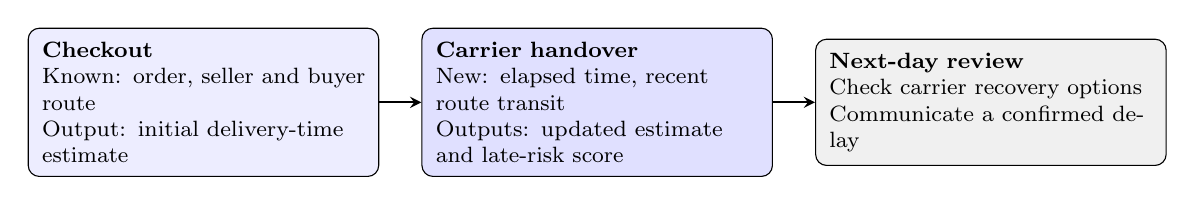
\begin{tikzpicture}[>=stealth,every node/.style={font=\footnotesize}]
\node[draw,rounded corners,fill=blue!7,align=left,text width=4.1cm,inner sep=5pt] (checkout) at (0,0) {\textbf{Checkout}\par Known: order, seller and buyer route\par Output: initial delivery-time estimate};
\node[draw,rounded corners,fill=blue!12,align=left,text width=4.1cm,inner sep=5pt] (handover) at (5.0,0) {\textbf{Carrier handover}\par New: elapsed time, recent route transit\par Outputs: updated estimate and late-risk score};
\node[draw,rounded corners,fill=gray!12,align=left,text width=4.1cm,inner sep=5pt] (action) at (10.0,0) {\textbf{Next-day review}\par Check carrier recovery options\par Communicate a confirmed delay};
\draw[->,thick] (checkout.east) -- (handover.west);
\draw[->,thick] (handover.east) -- (action.west);
\end{tikzpicture}
\caption{Prediction points and proposed action. Olist's original customer date anchors the late-risk label; delivery outcomes enter later model fits only after they are recorded.}
\label{fig:workflow}
\end{figure}

\section*{Model 1: the two-stage delivery-time estimate (regression)}
\textbf{Method.} Both stages predict the same target, \texttt{delivery\_days}, on the same orders; subtracting the already observed purchase-to-handover time from the handover prediction gives an estimate of remaining carrier days. The \textbf{checkout} stage uses the order, route and seller features known at purchase (20 inputs). The \textbf{handover} stage adds three inputs known once the carrier has the parcel: \texttt{handover\_days} (elapsed time), \texttt{approval\_days} (used only when approval was recorded by handover), and \texttt{route\_transit\_90d\_at\_handover} (the route's mean carrier-to-customer days over the previous 90 days, built only from deliveries already recorded, shrunk toward the all-route mean). Table~\ref{tab:ladder} holds ridge (\(\alpha=100\)) fixed while adding information; most of the improvement comes from observing elapsed time, while recent route history adds a smaller gain.

\begin{table}[ht]
\centering\small
\caption{Information ladder: ridge regression (\(\alpha=100\)) throughout, same orders at every rung, mean over five validation windows.}
\label{tab:ladder}
\begin{tabular}{@{}lrrr@{}}
\toprule
Rung & MAE (days) & \(R^2\) & Lowest-window \(R^2\) \\
\midrule
Checkout (20 frozen inputs) & \LadderCheckoutMAE{} & \LadderCheckoutRSq{} & \LadderCheckoutMinRSq{} \\
+ recent route transit history & \LadderTransitMAE{} & \LadderTransitRSq{} & \LadderTransitMinRSq{} \\
+ elapsed days to handover and approval & \LadderElapsedMAE{} & \LadderElapsedRSq{} & \LadderElapsedMinRSq{} \\
Handover (history as of handover) & \LadderHandoverMAE{} & \LadderHandoverRSq{} & \LadderHandoverMinRSq{} \\
\bottomrule
\end{tabular}
\end{table}

\textbf{Candidates and selection.} MAE is our selection measure because it expresses the average absolute miss in days; RMSE highlights larger errors and $R^2$ compares explained variation. We start with a training-mean floor, plain linear regression and a single tree, then test ridge penalties, tree pruning, random forest and gradient boosting. The latter two follow our Phase 1 review, but must earn their extra complexity on validation. At checkout, plain linear cuts MAE from the mean floor's \CheckoutMeanMAE{} to 5.86 days; ridge reaches \CheckoutSelMAE{}. A plain tree scores 7.79 days and improves to \CheckoutBestMAE{} with a forest. At handover, ridge improves on plain linear (5.15 to \HandoverSelMAE{} days), while the forest improves on the plain tree (6.84 to 5.35 days) but remains behind ridge.

Across families, we adapt the one-standard-error simplicity rule~\cite{james2013}: choose the lowest mean validation MAE unless a simpler model's \emph{paired} gap is within one standard error across the five windows. The checkout forest's advantage over ridge is only \CheckoutSelGap{} days (paired SE \CheckoutSelGapSE{}), so ridge $\alpha=100$ is selected there; at handover that ridge is itself the lowest-MAE candidate. An equal-weight ridge/boosting vote scores 5.11 days at handover, adding no improvement. The five windows make the SE approximate, but the selection does not depend on the opened test period. Full comparisons appear in Appendix Table~\ref{tab:app-regression}.

\begin{figure}[ht]
\centering
% BEGIN GENERATED fig_ladder -- refreshed by phase2_final_evidence.py
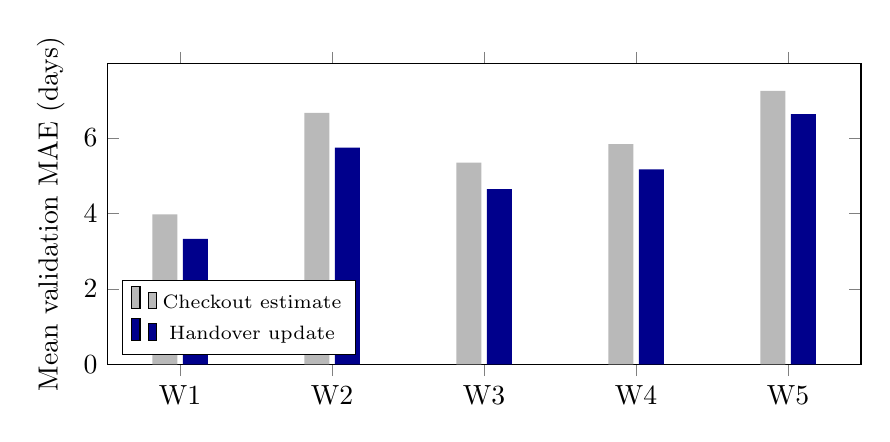
\begin{tikzpicture}
\begin{axis}[width=0.92\linewidth,height=5.4cm,ybar,bar width=9pt,ymin=0,ylabel={Mean validation MAE (days)},
 symbolic x coords={W1,W2,W3,W4,W5},xtick=data,enlarge x limits=0.12,legend style={at={(0.02,0.03)},anchor=south west,font=\scriptsize}]
\addplot[fill=gray!55,draw=none] coordinates {(W1,3.97) (W2,6.66) (W3,5.34) (W4,5.83) (W5,7.24)};
\addplot[fill=blue!55!black,draw=none] coordinates {(W1,3.32) (W2,5.74) (W3,4.64) (W4,5.16) (W5,6.63)};
\legend{Checkout estimate,Handover update}
\end{axis}
\end{tikzpicture}
% END GENERATED fig_ladder
\caption{Mean validation MAE by window, checkout estimate against the handover update (selected models). The handover update beats the checkout estimate in every window, including the higher-lateness windows.}
\label{fig:ladder}
\end{figure}

\textbf{Later-period results.} On the later period, the selected checkout fit has MAE \CheckoutTestMAE{}, RMSE \CheckoutTestRMSE{} and \(R^2\) \CheckoutTestRSq{}; the handover update has MAE \HandoverTestMAE{}, RMSE \HandoverTestRMSE{} and \(R^2\) \HandoverTestRSq{}. The update still lowers the average absolute miss, by about one day. Both fits predict later arrival than actually occurred in this faster period, with mean signed errors of \CheckoutTestBias{} and \HandoverTestBias{} days (Appendix Figure~\ref{fig:test-bias}). A lower MAE than on validation can coexist with negative checkout \(R^2\): the latter compares the fit with the later period's own mean. The bias reinforces using this point estimate as review context rather than issuing it as a new customer date.

\textbf{What drives the estimate.} Among scaled numeric and engineered inputs, the largest mean absolute ridge coefficients at checkout are \texttt{\CheckoutImpAName{}} (\CheckoutImpAVal{}), \texttt{\CheckoutImpBName{}} (\CheckoutImpBVal{}) and \texttt{\CheckoutImpCName{}} (\CheckoutImpCVal{}). At handover, observed elapsed time (\texttt{\HandoverImpAName{}}; \HandoverImpAVal{}) leads. This matches the information ladder: knowing how long the order has already taken is the main reason to update its estimate. Correlated inputs and omitted one-hot categories mean coefficient magnitudes describe the fitted model, not isolated causal effects.

\section*{Model 2: the late warning (classification)}
\textbf{Candidates and selection.} We start with unregularised logistic regression (mean validation PR-AUC \ClsPlainPR{}) and a plain tree (0.138), then test regularisation, class weights, pruned trees, forests and boosting. The selected logistic fit at $C=0.01$ raises PR-AUC to \ValSelPR{}; class weighting lowers it to 0.350, so fitting retains the natural late-order frequency. The best forest reaches \ValBestPR{}, only \ClsSelGap{} above logistic, a gap smaller than its paired one-SE estimate (\ClsSelGapSE{}). We therefore select the simpler logistic fit rather than claim a meaningful forest advantage. The full family comparisons appear in Appendix Table~\ref{tab:app-classifier}.

\textbf{Imbalance and metrics.} Only \ClsTestLate{}\% of test orders are late (4--21\% across validation windows), so accuracy would obscure the minority class. We select by PR-AUC (average precision) and show each period's late rate as its random-ranking baseline~\cite{saito2015}. We also report ROC-AUC for discrimination and precision, recall and F1 at a review share to show what a review queue would identify. Appendix Figure~\ref{fig:roc-pr} shows ROC and precision--recall curves; Appendix Table~\ref{tab:app-confusion} gives confusion counts and MCC at the validation-selected 14\% monthly review share.

Table~\ref{tab:classifier-windows} shows why the mean score is insufficient: late prevalence and top-10\% precision change sharply, but that precision exceeds the late rate in every window and ROC-AUC remains between 0.74 and 0.82. The model concentrates late orders even when conditions change; a fixed-size queue nevertheless yields a different number of useful reviews in each period. The 10\% share is a common comparison point, with any operating share considered separately below.

% BEGIN GENERATED fig_classifier_windows -- refreshed by phase2_final_evidence.py
\begin{table}[ht]
\centering\small
\caption{Selected classifier across chronological validation windows. Each late rate is the no-skill PR-AUC baseline; top-10\% precision is an offline ranking measure.}
\label{tab:classifier-windows}
\begin{tabular}{@{}lrrrrr@{}}
\toprule
Window & Orders & Late rate & PR-AUC & ROC-AUC & Top-10\% precision \\
\midrule
W1 & 7,600 & 4.1\% & 0.333 & 0.817 & 21.2\% \\
W2 & 7,601 & 13.8\% & 0.409 & 0.757 & 44.8\% \\
W3 & 7,601 & 4.8\% & 0.265 & 0.743 & 16.3\% \\
W4 & 7,601 & 9.9\% & 0.354 & 0.778 & 35.1\% \\
W5 & 7,600 & 20.7\% & 0.472 & 0.752 & 56.6\% \\
\bottomrule
\end{tabular}
\end{table}
% END GENERATED fig_classifier_windows

\textbf{Ranking on the later period.} The selected model's PR-AUC is \ClsTestPR{} against the period's \ClsTestLate{}\% no-skill baseline, with ROC-AUC \ClsTestROC{}. In retrospective purchase-month ranking, the top 10\% contains \GainTenModel{}\% of late orders, against 10\% under random selection (Figure~\ref{fig:gains}). This is a useful concentration of risk for a limited review queue; it does not determine how many orders staff should review.

\textbf{Operating point.} To examine a workload choice, we compared review shares from 1\% to 30\% in one-point steps rather than relying on a probability cutoff across changing periods. We assigned \BenefitRatio{} units to each late order identified and charged one unit per review. This is an assumed tradeoff, not an observed cost or recovery benefit. It selects the top \ActShare{}\% on validation; two-to-one selects 1\%, while ten-to-one selects 30\%, the largest share tested. The sensitivity makes staffing capacity a business decision rather than a property of the classifier.

Validation ranks within each completed window; the test calculation applies that same share within each completed purchase month. Those groupings use future scores, so the action metrics below are \emph{retrospective ranking measures}; the separate daily replay estimates workload when the same share is applied by handover day.

\begin{table}[ht]
\centering\small
\caption{Opened-test discrimination and retrospective top-\ActShare{}\% review results within purchase month. PR-AUC and ROC-AUC use all scores; precision, recall and F1 use the selected share.}
\label{tab:classifier-test}
\begin{tabular}{@{}lccccc@{}}
\toprule
& PR-AUC & ROC-AUC & Precision & Recall & F1 \\
\midrule
Late-warning model & \ClsTestPR{} & \ClsTestROC{} & \ClsTestPrec{}\% & \ClsTestRec{}\% & \ClsTestFone{} \\
Random list & \ClsTestLate{}\% & 0.50 & \ClsTestLate{}\% & \ActShare{}\% & --- \\
\bottomrule
\end{tabular}
\end{table}

\textbf{Later-period decision check.} At the validation-selected \ActShare{}\% share, precision is \ClsTestPrec{}\% (Table~\ref{tab:classifier-test}). The assumed five-to-one score requires at least 20\% precision to offset one unit per review, so this share scores \ClsNetBenefit{} per order, below zero for reviewing none. The fixed share is too broad under this tradeoff; operations should set pilot capacity using actual review costs and recovery options. Appendix Table~\ref{tab:classifier-monthly} gives the purchase-month counts.

\textbf{Daily replay: workload and timing.} Monthly ranking uses future scores from a completed purchase month, so we also replayed the selected model at each day's valid handovers in the later calendar span, retaining \ActShare{}\% only as a workload illustration. This broader handover-day cohort includes purchases outside the monthly test cohort. Of \FullDailyOrders{} handovers, \FullDailyFlagged{} were flagged and \FullDailyCaught{} of \FullDailyLate{} late orders identified (\FullDailyPrecision{}\% precision; \FullDailyRecall{}\% recall). The median queue was \FullDailyMedianFlagged{} orders per active day (90th percentile \FullDailyPninetyFlagged{}). By 09:00 the next morning, \FullDailyBeforePromise{} identified late orders were still undelivered and before their promised date, leaving a possible response window; \FullDailyExpiredCaught{} had already missed it. A next-day review could therefore begin before the date for some flagged orders, but not all (Appendix Table~\ref{tab:daily-replay}).

% BEGIN GENERATED fig_split_summary -- refreshed by phase2_final_evidence.py
\begin{table}[ht]
\centering\small
\caption{Selected-model train--validate--test comparison. Train is apparent, in-sample fit; validation is the mean of five chronological windows; the previously inspected test describes later conditions. Periods and late prevalence differ.}
\label{tab:split-summary}
\begin{tabular}{@{}lrrr@{}}
\toprule
Metric & Train (apparent) & Validation & Later test \\
\midrule
Checkout MAE (days) & 5.23 & 5.81 & 5.00 \\
Handover MAE (days) & 4.57 & 5.10 & 3.97 \\
Late warning PR-AUC & 0.333 & 0.367 & 0.231 \\
Late prevalence & 7.1\% & 10.7\% & 3.5\% \\
\bottomrule
\end{tabular}
\end{table}
% END GENERATED fig_split_summary

Table~\ref{tab:split-summary} puts the selected fits in context. The handover regression has lower MAE than checkout on the apparent train fit, every validation window (Figure~\ref{fig:ladder}) and the later period. Classifier PR-AUC falls from \ValSelPR{} to \ClsTestPR{} while the late rate falls from 10.7\% to \ClsTestLate{}\%; lower prevalence tends to reduce precision even when ranking remains useful. ROC-AUC instead rises from \ValSelROC{} to \ClsTestROC{}, so these results do not show a loss of discrimination. The training scores are apparent fit on a different outcome mix, not a substitute for time-ordered validation.

\begin{figure}[ht]
\centering
% BEGIN GENERATED fig_gains -- refreshed by phase2_final_evidence.py
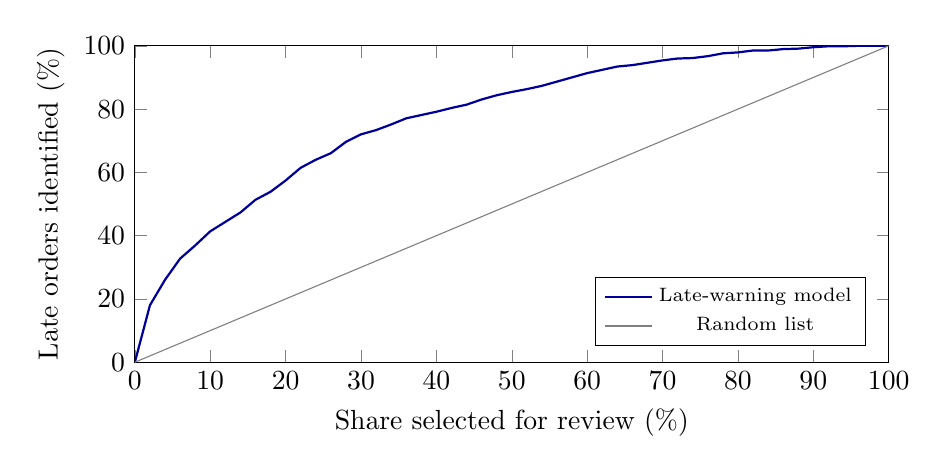
\begin{tikzpicture}
\begin{axis}[width=0.92\linewidth,height=5.6cm,xlabel={Share selected for review (\%)},ylabel={Late orders identified (\%)},
 xmin=0,xmax=100,ymin=0,ymax=100,legend style={at={(0.97,0.05)},anchor=south east,font=\scriptsize}]
\addplot[thick,blue!60!black,no marks] coordinates {(0.0,0.0000) (2.0,18.0060) (4.0,26.0417) (6.0,32.7381) (8.0,36.9048) (10.0,41.3690) (12.0,44.3452) (14.000000000000002,47.3214) (16.0,51.3393) (18.0,53.8690) (20.0,57.4405) (22.0,61.4583) (24.0,63.9881) (26.0,66.0714) (28.000000000000004,69.6429) (30.0,72.0238) (32.0,73.3631) (34.0,75.1488) (36.0,77.0833) (38.0,78.1250) (40.0,79.1667) (42.0,80.3571) (44.0,81.3988) (46.0,83.0357) (48.0,84.3750) (50.0,85.4167) (52.0,86.3095) (54.0,87.3512) (56.00000000000001,88.6905) (57.99999999999999,90.0298) (60.0,91.3690) (62.0,92.4107) (64.0,93.4524) (66.0,93.8988) (68.0,94.6429) (70.0,95.3869) (72.0,95.9821) (74.0,96.1310) (76.0,96.7262) (78.0,97.6190) (80.0,97.9167) (82.0,98.5119) (84.0,98.5119) (86.0,98.9583) (88.0,99.1071) (90.0,99.5536) (92.0,99.8512) (94.0,99.8512) (96.0,100.0000) (98.0,100.0000) (100.0,100.0000)};
\addlegendentry{Late-warning model}
\addplot[thin,gray,no marks] coordinates {(0.0,0.0000) (2.0,2.0000) (4.0,4.0000) (6.0,6.0000) (8.0,8.0000) (10.0,10.0000) (12.0,12.0000) (14.000000000000002,14.0000) (16.0,16.0000) (18.0,18.0000) (20.0,20.0000) (22.0,22.0000) (24.0,24.0000) (26.0,26.0000) (28.000000000000004,28.0000) (30.0,30.0000) (32.0,32.0000) (34.0,34.0000) (36.0,36.0000) (38.0,38.0000) (40.0,40.0000) (42.0,42.0000) (44.0,44.0000) (46.0,46.0000) (48.0,48.0000) (50.0,50.0000) (52.0,52.0000) (54.0,54.0000) (56.00000000000001,56.0000) (57.99999999999999,58.0000) (60.0,60.0000) (62.0,62.0000) (64.0,64.0000) (66.0,66.0000) (68.0,68.0000) (70.0,70.0000) (72.0,72.0000) (74.0,74.0000) (76.0,76.0000) (78.0,78.0000) (80.0,80.0000) (82.0,82.0000) (84.0,84.0000) (86.0,86.0000) (88.0,88.0000) (90.0,90.0000) (92.0,92.0000) (94.0,94.0000) (96.0,96.0000) (98.0,98.0000) (100.0,100.0000)};
\addlegendentry{Random list}
\end{axis}
\end{tikzpicture}
% END GENERATED fig_gains
\caption{Opened-test gain curve under retrospective purchase-month ranking; it measures ordering quality, not day-by-day action.}
\label{fig:gains}
\end{figure}

\textbf{What drives the score.} We adapt Breiman's permutation-importance idea~\cite{breiman2001} to validation PR-AUC: the reported drop is the change when a column is shuffled. It is led by \texttt{\ImpAName{}} (\ImpADrop{}), then \texttt{\ImpBName{}} (\ImpBDrop{}) and \texttt{\ImpCName{}} (\ImpCDrop{}); all other inputs contribute under 0.02 each. The model reads mainly the time already spent against the promised date, which explains why handover is a useful moment to reassess risk.

\section*{Proposed operations workflow}
\begin{enumerate}\setlength{\itemsep}{0pt}
\item \textbf{At carrier handover}, score risk against Olist's existing customer date and update the estimate of remaining delivery time. Rank that day's handovers for the next review cycle.
\item \textbf{Within a pilot capacity set by operations}, open the highest-risk cases and show staff the remaining-time estimate. For each, ask the carrier whether a faster feasible service or recovery action exists and what it costs. If a delay is confirmed and cannot be recovered, give the customer a verified update.
\item \textbf{Across periods}, monitor forecast error, late prevalence, queue precision and actual review workload before changing capacity.
\end{enumerate}

\section*{Limitations and pilot requirements}
\begin{itemize}\setlength{\itemsep}{0pt}
\item \textbf{Conditions change.} About \NormalLate{}\% of orders are late in ordinary months, against \BlackFridayLate{}\% around Black Friday and \FebMarLate{}\% in February--March 2018 (Appendix Figure~\ref{fig:monthly}). A review capacity suited to one period may not suit another.
\item \textbf{Cohort.} Results describe orders that were eventually delivered with a recorded carrier handover; cancelled and still-open orders have no outcome and are not covered.
\item \textbf{Intervention outcomes.} Olist's data do not record carrier recovery options, their costs, or effects on delivery and reviews. A pilot with a control group would test whether acting on the scores improves outcomes enough to justify its cost.
\end{itemize}

\section*{Declaration on the use of AI}
Claude (Anthropic) and OpenAI Codex assisted with analysis code, figures and report drafting. The student authors are responsible for checking the calculations, citations and final submission.

\begin{thebibliography}{99}\small\setlength{\itemsep}{0pt}
\bibitem{bergmeir2012} C.~Bergmeir and J.~M.~Ben\'itez. On the use of cross-validation for time series predictor evaluation. \emph{Information Sciences}, 2012. doi:10.1016/j.ins.2011.12.028.
\bibitem{breiman2001} L.~Breiman. Random forests. \emph{Machine Learning}, 45(1):5--32, 2001.
\bibitem{dearaujo2021} A.~C.~de Araujo and A.~Etemad. End-to-end prediction of parcel delivery time with deep learning for smart-city applications. \emph{IEEE Internet of Things Journal}, 8(23):17043--17056, 2021. doi:10.1109/JIOT.2021.3077007.
\bibitem{gibellini2024} F.~Gibellini, B.~van Gool, M.~Firat and S.~Bromuri. Estimating the time of arrival of a shipment with machine learning. \emph{ECAI 2024}, pp.~4681--4688. doi:10.3233/FAIA241064.
\bibitem{james2013} G.~James, D.~Witten, T.~Hastie and R.~Tibshirani. \emph{An Introduction to Statistical Learning}, Sec.~6.1.3, p.~214. Springer, 2013.
\bibitem{saito2015} T.~Saito and M.~Rehmsmeier. The precision-recall plot is more informative than the ROC plot when evaluating binary classifiers on imbalanced datasets. \emph{PLOS ONE}, 10(3):e0118432, 2015.
\bibitem{salari2022} N.~Salari, S.~Liu and Z.-J.~M.~Shen. Real-time delivery time forecasting and promising in online retailing: when will your package arrive? \emph{Manufacturing \& Service Operations Management}, 24(3):1421--1436, 2022.
\end{thebibliography}

\clearpage
\appendix
\section{Prepared-table validation}
\label{app:gx}
Before the delivery-sequence exclusions, a Great Expectations (GX Core 1.24.0) suite checked the 96,470-row prepared order table. Its saved run passed all 35 expectations: eight identity, target and split checks; one exact-column-set check; 16 value-range checks; five category checks; and five missingness checks. Separate timestamp checks confirmed that fitting outcomes were recorded by the 26 May 2018 cutoff. The model comparison uses 96,272 orders after excluding 198 rows without a valid purchase--carrier--delivery sequence.

\begin{table}[ht]
\centering\small
\caption{Prepared-table validation and later-period feature checks. The 35 contract checks apply before the final sequence filter; monthly feature checks are separate diagnostics.}
\label{tab:gx}
\begin{tabular}{@{}lr@{}}
\toprule
Check & Saved result \\
\midrule
Identity, targets and split & 8/8 passed \\
Exact column set & 1/1 passed \\
Value ranges and categories & 21/21 passed \\
Documented missingness & 5/5 passed \\
Later monthly feature means outside training range & 5 of 21 \\
\bottomrule
\end{tabular}
\end{table}

The five out-of-range means are June freight, July promised days and freight, and August promised days and historical seller handover time. They document a change in the observed feature mix, not its cause. An exact column set can catch an unapproved predictor, but cannot establish when a historical value became known; the point-in-time feature construction is checked separately.

\section{Delivery context and diagnostics}
\begin{table}[H]
\centering\small
\caption{Retrospective purchase-month test ranking at the validation-selected \ActShare{}\% share. Counts describe model selection for review, not carrier interventions.}
\label{tab:classifier-monthly}
\begin{tabular}{@{}lrrrr@{}}
\toprule
Month & Orders & Late orders & Flagged & Late caught \\
\midrule
May (from the 26th) & \TestMayOrders{} & \TestMayLateCount{} & \TestMayActed{} & \TestMayCaught{} \\
June & \TestJunOrders{} & \TestJunLateCount{} & \TestJunActed{} & \TestJunCaught{} \\
July & \TestJulOrders{} & \TestJulLateCount{} & \TestJulActed{} & \TestJulCaught{} \\
August & \TestAugOrders{} & \TestAugLateCount{} & \TestAugActed{} & \TestAugCaught{} \\
\bottomrule
\end{tabular}
\end{table}
% BEGIN GENERATED fig_complete_daily_replay -- refreshed by phase2_final_evidence.py
\begin{table}[H]
\centering\small
\caption{Complete handover-day replay at the fixed validation-selected model and 14\% review share. Each row contains all valid handovers in its calendar span, including purchases outside the original purchase-window scoring cohort. The later-period analysis was specified after that period had been inspected. Workload is per active handover day; results do not measure intervention effects.}
\label{tab:daily-replay}
\begin{tabular}{@{}lrrrrrr@{}}
\toprule
Period & Active days & Orders & Late rate & Median flagged/day & Precision & Recall \\
\midrule
W1 & 45 & 7,262 & 3.6\% & 27 & 13.7\% & 54.0\% \\
W2 & 24 & 7,450 & 12.9\% & 50 & 34.9\% & 38.3\% \\
W3 & 33 & 7,685 & 5.7\% & 37 & 18.6\% & 46.5\% \\
W4 & 28 & 7,591 & 9.1\% & 46 & 25.9\% & 40.4\% \\
W5 & 29 & 7,357 & 21.9\% & 41 & 53.8\% & 34.9\% \\
Later period & 81 & 19,534 & 3.6\% & 38 & 12.5\% & 49.2\% \\
\bottomrule
\end{tabular}
\end{table}
% END GENERATED fig_complete_daily_replay
\textbf{Same-period diagnostic.} A secondary random five-fold validation and 20\% test yield checkout \(R^2\) \CheckoutRandValRSq{} / \CheckoutRandTestRSq{} (test MAE \CheckoutRandTestMAE{}) and handover \(R^2\) \HandoverRandValRSq{} / \HandoverRandTestRSq{} (test MAE \HandoverRandTestMAE{}). These interpolate within one period and were not used for model selection; their stronger scores illustrate the cost of temporal shift.
\begin{figure}[H]
\centering
% BEGIN GENERATED fig_monthly -- refreshed by phase2_final_evidence.py
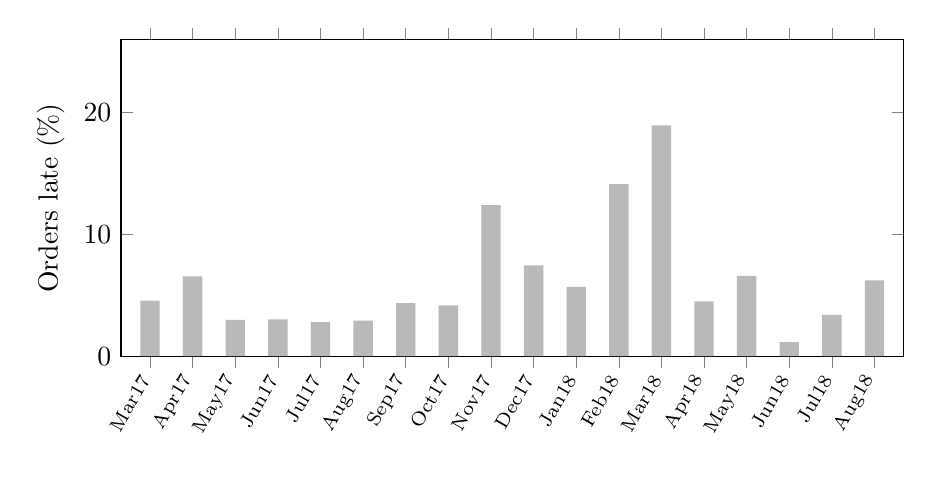
\begin{tikzpicture}
\begin{axis}[width=0.95\linewidth,height=5.6cm,ybar,bar width=7pt,ymin=0,ymax=26,ylabel={Orders late (\%)},
 symbolic x coords={Mar17,Apr17,May17,Jun17,Jul17,Aug17,Sep17,Oct17,Nov17,Dec17,Jan18,Feb18,Mar18,Apr18,May18,Jun18,Jul18,Aug18},xtick=data,x tick label style={rotate=60,anchor=east,font=\scriptsize},
 enlarge x limits=0.04]
\addplot[fill=gray!55,draw=none] coordinates {(Mar17,4.558) (Apr17,6.557) (May17,2.991) (Jun17,3.031) (Jul17,2.799) (Aug17,2.912) (Sep17,4.362) (Oct17,4.176) (Nov17,12.404) (Dec17,7.455) (Jan18,5.701) (Feb18,14.127) (Mar18,18.966) (Apr18,4.506) (May18,6.593) (Jun18,1.157) (Jul18,3.383) (Aug18,6.232)};
\end{axis}
\end{tikzpicture}
% END GENERATED fig_monthly
\caption{Share of orders late by purchase month. Black Friday (November 2017) and February--March 2018 stand out as the clearest swings in delivery conditions; the June--August 2018 test months at right were calmer at \ClsTestLate{}\% late.}
\label{fig:monthly}
\end{figure}


\begin{figure}[H]
\centering
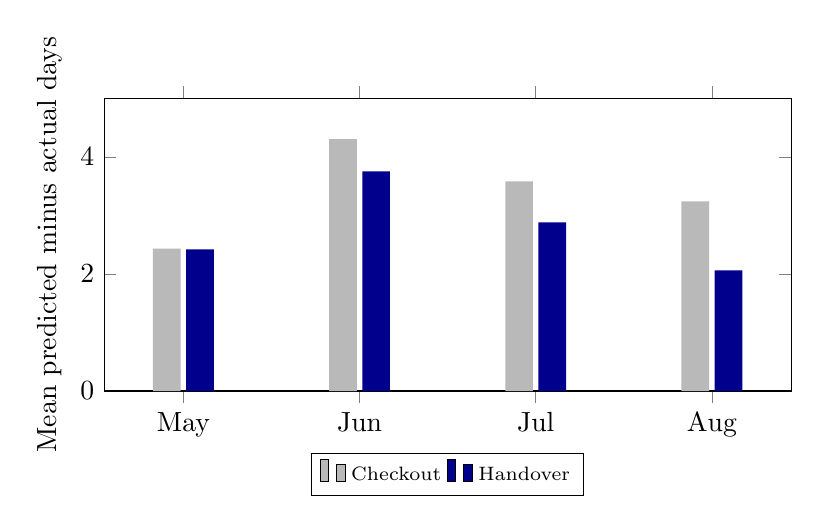
\begin{tikzpicture}
\begin{axis}[width=0.85\linewidth,height=5.3cm,ybar,bar width=10pt,ymin=0,ymax=5,
 symbolic x coords={May,Jun,Jul,Aug},xtick=data,enlarge x limits=0.15,
 ylabel={Mean predicted minus actual days},
 legend style={at={(0.5,-0.21)},anchor=north,legend columns=2,font=\scriptsize}]
\addplot[fill=gray!55,draw=none] coordinates {(May,2.43) (Jun,4.30) (Jul,3.58) (Aug,3.24)};
\addplot[fill=blue!55!black,draw=none] coordinates {(May,2.42) (Jun,3.75) (Jul,2.88) (Aug,2.06)};
\legend{Checkout,Handover}
\end{axis}
\end{tikzpicture}
\caption{Signed forecast error by purchase month in the later test period (May starts on the 26th). Positive values mean predicted delivery is later than actual delivery. This diagnoses the shift to faster deliveries; it was not used for model selection.}
\label{fig:test-bias}
\end{figure}

\begin{figure}[H]
\centering
\begin{minipage}{0.49\linewidth}\centering
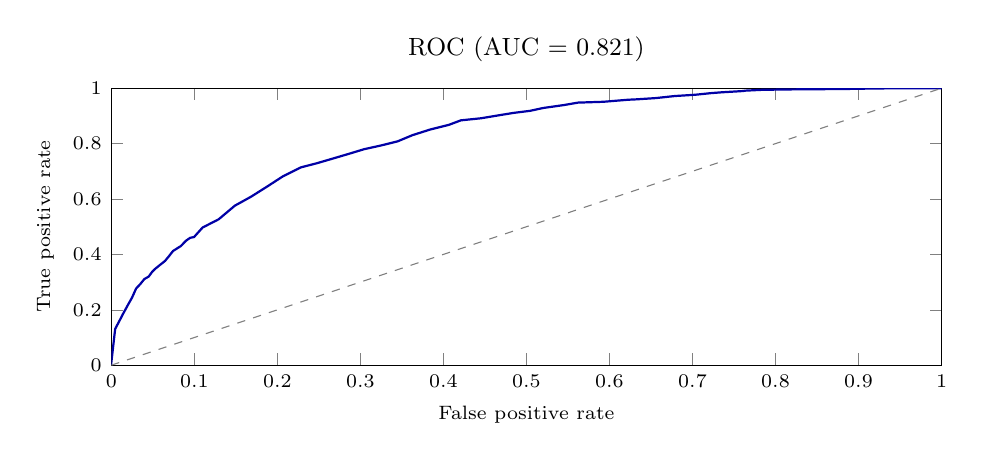
\begin{tikzpicture}
\begin{axis}[width=\linewidth,height=5.1cm,xmin=0,xmax=1,ymin=0,ymax=1,
 xlabel={False positive rate},ylabel={True positive rate},
 title={ROC (AUC = 0.821)},title style={font=\small},tick label style={font=\scriptsize},label style={font=\scriptsize}]
\addplot[thick,blue!65!black,no marks] coordinates {(0.00000,0.00000) (0.00000,0.00893) (0.00463,0.13095) (0.00986,0.16071) (0.01450,0.18750) (0.01994,0.21726) (0.02495,0.24405) (0.02985,0.27679) (0.03497,0.29315) (0.03977,0.31101) (0.04499,0.31994) (0.04936,0.33780) (0.05351,0.34970) (0.05970,0.36458) (0.06472,0.37649) (0.06924,0.39286) (0.07431,0.41220) (0.07970,0.42262) (0.08374,0.43006) (0.08993,0.44940) (0.09495,0.45982) (0.09969,0.46280) (0.10993,0.49702) (0.12932,0.52679) (0.14878,0.57589) (0.16850,0.60863) (0.18817,0.64583) (0.20654,0.68155) (0.22847,0.71429) (0.24771,0.72917) (0.26802,0.74702) (0.28651,0.76339) (0.30445,0.77976) (0.32477,0.79315) (0.34481,0.80804) (0.36265,0.83036) (0.38452,0.85119) (0.40646,0.86756) (0.42106,0.88393) (0.44525,0.89137) (0.46002,0.89881) (0.48427,0.91071) (0.50420,0.91815) (0.52026,0.92857) (0.54494,0.93899) (0.56218,0.94792) (0.57727,0.94940) (0.59268,0.95089) (0.62259,0.95833) (0.63310,0.95982) (0.65589,0.96429) (0.67890,0.97173) (0.70304,0.97619) (0.72228,0.98214) (0.73510,0.98512) (0.76016,0.98958) (0.76366,0.99107) (0.78371,0.99405) (0.81501,0.99554) (0.88145,0.99702) (0.91077,0.99851) (0.95140,1.00000) (1.00000,1.00000)};
\addplot[thin,gray,dashed,no marks] coordinates {(0,0) (1,1)};
\end{axis}
\end{tikzpicture}
\end{minipage}\hfill
\begin{minipage}{0.49\linewidth}\centering
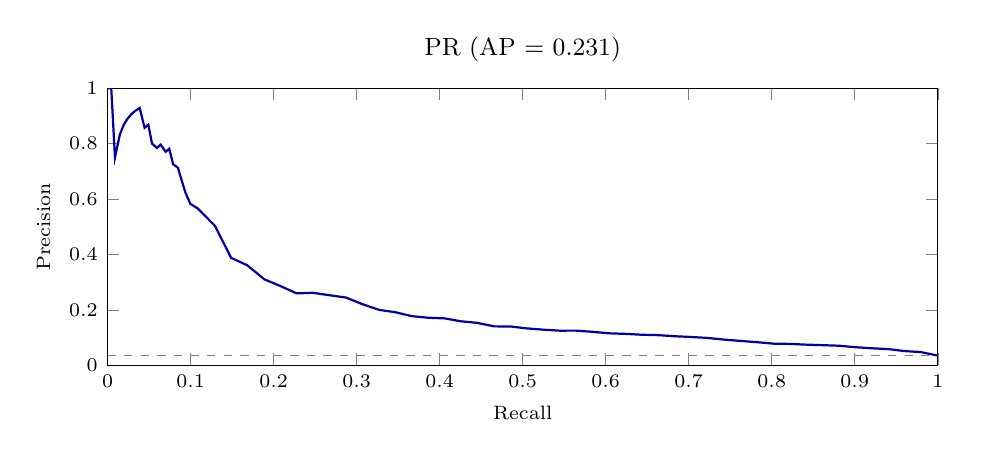
\begin{tikzpicture}
\begin{axis}[width=\linewidth,height=5.1cm,xmin=0,xmax=1,ymin=0,ymax=1,
 xlabel={Recall},ylabel={Precision},
 title={PR (AP = 0.231)},title style={font=\small},tick label style={font=\scriptsize},label style={font=\scriptsize}]
\addplot[thick,blue!65!black,no marks] coordinates {(0.00000,1.00000) (0.00446,1.00000) (0.00893,0.75000) (0.01488,0.83333) (0.01935,0.86667) (0.02381,0.88889) (0.02976,0.90909) (0.03423,0.92000) (0.03869,0.92857) (0.04464,0.85714) (0.04911,0.86842) (0.05357,0.80000) (0.05952,0.78431) (0.06399,0.79630) (0.06994,0.77049) (0.07440,0.78125) (0.07887,0.72603) (0.08482,0.71250) (0.08929,0.66667) (0.09375,0.62376) (0.09970,0.58261) (0.10863,0.56589) (0.12946,0.50289) (0.14881,0.38760) (0.16815,0.36102) (0.18899,0.30976) (0.20833,0.28571) (0.22768,0.25932) (0.24702,0.26142) (0.26786,0.25245) (0.28720,0.24430) (0.30655,0.22079) (0.32738,0.19964) (0.34673,0.19130) (0.36607,0.17736) (0.38542,0.17152) (0.40625,0.16904) (0.42560,0.15862) (0.44494,0.15294) (0.46577,0.14023) (0.48512,0.13997) (0.50446,0.13315) (0.52530,0.12822) (0.54464,0.12474) (0.56399,0.12496) (0.58333,0.12073) (0.60417,0.11518) (0.62351,0.11321) (0.64286,0.11009) (0.66369,0.10846) (0.68304,0.10465) (0.70238,0.10205) (0.72173,0.09870) (0.74256,0.09253) (0.76190,0.08784) (0.78125,0.08341) (0.80208,0.07788) (0.82143,0.07701) (0.84077,0.07436) (0.86012,0.07252) (0.88095,0.07043) (0.90030,0.06510) (0.91964,0.06129) (0.94048,0.05825) (0.95982,0.05111) (0.97917,0.04754) (1.00000,0.03495)};
\addplot[thin,gray,dashed,no marks] coordinates {(0,0.0349454) (1,0.0349454)};
\end{axis}
\end{tikzpicture}
\end{minipage}
\caption{Final handover logistic classifier on 19,230 test orders (672 late). Curves are sampled points for display; AUC and average precision (AP) are calculated from all predictions. The dashed lines show random ranking. The top-14\% review policy is applied separately by month and therefore has no single operating point on these pooled curves.}
\label{fig:roc-pr}
\end{figure}

\begin{table}[H]
\centering\small
\caption{Test confusion counts at the validation-selected top-14\% monthly review share. These are ranking outcomes, before any carrier intervention.}
\label{tab:app-confusion}
\begin{tabular}{@{}lrr@{}}
\toprule
& Actually late & Actually on time \\
\midrule
Selected for review & 318 & 2375 \\
Not selected & 354 & 16183 \\
\bottomrule
\end{tabular}
\end{table}

At this review share, MCC is \ClsTestMCC{} (zero indicates no association between selection and lateness).

\section{Full configuration tables}
% BEGIN GENERATED fig_appendix_regression -- refreshed by phase2_final_evidence.py
\begin{table}[H]
\centering\small
\caption{Every regression candidate, mean over five validation windows.}
\label{tab:app-regression}
\begin{tabular}{@{}lllrrr@{}}
\toprule
Stage & Candidate & Family & MAE & RMSE & $R^2$ \\
\midrule
Checkout & mean\_baseline & mean & 7.215 & 10.671 & -0.078 \\
Checkout & linear\_baseline & linear & 5.860 & 9.464 & 0.155 \\
Checkout & ridge\_1 & ridge & 5.858 & 9.462 & 0.156 \\
Checkout & ridge\_10 & ridge & 5.848 & 9.451 & 0.158 \\
Checkout & ridge\_100 & ridge & 5.809 & 9.398 & 0.167 \\
Checkout & tree\_baseline & tree & 7.787 & 12.344 & -0.472 \\
Checkout & tree\_depth6 & tree & 5.933 & 9.505 & 0.144 \\
Checkout & forest\_leaf20 & forest & 5.783 & 9.340 & 0.176 \\
Checkout & boost\_baseline & boost & 5.830 & 9.452 & 0.155 \\
Checkout & boost\_slow & boost & 5.816 & 9.444 & 0.157 \\
Handover & mean\_baseline & mean & 7.215 & 10.671 & -0.078 \\
Handover & elapsed\_plus\_route\_baseline & rule & 5.304 & 8.396 & 0.337 \\
Handover & linear\_baseline & linear & 5.146 & 8.472 & 0.327 \\
Handover & ridge\_1 & ridge & 5.145 & 8.470 & 0.327 \\
Handover & ridge\_10 & ridge & 5.136 & 8.460 & 0.329 \\
Handover & ridge\_100 & ridge & 5.099 & 8.406 & 0.338 \\
Handover & tree\_baseline & tree & 6.840 & 11.625 & -0.330 \\
Handover & tree\_depth6 & tree & 5.313 & 8.633 & 0.299 \\
Handover & forest\_leaf20 & forest & 5.346 & 8.808 & 0.270 \\
Handover & boost\_baseline & boost & 5.214 & 8.651 & 0.297 \\
Handover & boost\_slow & boost & 5.215 & 8.666 & 0.294 \\
Handover & voting\_family\_winners & voting & 5.107 & 8.471 & 0.327 \\
\bottomrule
\end{tabular}
\end{table}
% END GENERATED fig_appendix_regression
% BEGIN GENERATED fig_appendix_classifier -- refreshed by phase2_final_evidence.py
\begin{table}[H]
\centering\small
\caption{Every classifier candidate, mean over five validation windows (handover stage).}
\label{tab:app-classifier}
\begin{tabular}{@{}lrrr@{}}
\toprule
Candidate & PR-AUC & ROC-AUC & Recall at top 10\% \\
\midrule
logistic\_unregularized & 0.337 & 0.733 & 0.344 \\
logistic\_c1 & 0.343 & 0.739 & 0.349 \\
logistic\_c1\_bal & 0.328 & 0.734 & 0.338 \\
logistic\_c0.01 & 0.367 & 0.769 & 0.363 \\
logistic\_c0.01\_bal & 0.350 & 0.761 & 0.350 \\
logistic\_c0.1 & 0.354 & 0.755 & 0.355 \\
logistic\_c0.1\_bal & 0.337 & 0.743 & 0.343 \\
logistic\_c10 & 0.338 & 0.733 & 0.345 \\
logistic\_c10\_bal & 0.325 & 0.730 & 0.335 \\
tree\_plain & 0.138 & 0.561 & 0.213 \\
tree\_d4\_l20 & 0.283 & 0.667 & 0.287 \\
tree\_d4\_l100 & 0.280 & 0.667 & 0.286 \\
tree\_d6\_l20 & 0.302 & 0.692 & 0.313 \\
tree\_d6\_l100 & 0.306 & 0.700 & 0.321 \\
tree\_d8\_l20 & 0.306 & 0.694 & 0.297 \\
tree\_d8\_l100 & 0.308 & 0.684 & 0.322 \\
tree\_d12\_l20 & 0.290 & 0.632 & 0.294 \\
tree\_d12\_l100 & 0.302 & 0.663 & 0.309 \\
forest\_l5\_sqrt & 0.360 & 0.735 & 0.338 \\
forest\_l5\_half & 0.344 & 0.723 & 0.319 \\
forest\_l20\_sqrt & 0.366 & 0.745 & 0.341 \\
forest\_l20\_half & 0.354 & 0.733 & 0.339 \\
forest\_l50\_sqrt & 0.369 & 0.747 & 0.343 \\
forest\_l50\_half & 0.357 & 0.737 & 0.344 \\
boost\_lr0.03\_n200\_l20 & 0.354 & 0.741 & 0.333 \\
boost\_lr0.03\_n200\_l100 & 0.345 & 0.739 & 0.329 \\
boost\_lr0.03\_n500\_l20 & 0.344 & 0.731 & 0.320 \\
boost\_lr0.03\_n500\_l100 & 0.333 & 0.729 & 0.318 \\
boost\_lr0.1\_n200\_l20 & 0.334 & 0.722 & 0.312 \\
boost\_lr0.1\_n200\_l100 & 0.330 & 0.719 & 0.309 \\
boost\_lr0.1\_n500\_l20 & 0.318 & 0.702 & 0.299 \\
boost\_lr0.1\_n500\_l100 & 0.318 & 0.703 & 0.300 \\
\bottomrule
\end{tabular}
\end{table}
% END GENERATED fig_appendix_classifier

\end{document}
